\section{January 2021}
    {\sffamily{Mechanics, Position/Location Denote-rs, Notations, Conditions, Proofs, Prime Numbers, Particles, Constraints, Connections, Arrows, Diagrams, Chocolate, Conservation, Spaces, Additions, Multiplications, Conventions, Civil Engineering (Just Joking), Pulleys, Planes, Exam Centers, Geometry and What Not?}}
\thispagestyle{empty}
\newpage
%------------------------------------------------------------
\begin{mathbox}{\text{\subsection{A Simple Proof}}}
{Are there infinitely many prime numbers? If yes, how do we prove they exist?\\
Here's a simple proof.\\
{Assume} we have only $n$ prime numbers; $P_1, P_2, P_3, \dots P_n$.
\begin{align*}
\text{Let}~N = P_1 \cdot P_2 \cdot P_3 \dots P_n + 1
\end{align*}
$N$ {isn't divisible} by any of the primes $P_1, P_2, P_3, \dots P_n$\footnote{Prime numbers start from $2$ and $N$ is the LCM of all the prime numbers added to $1$.}  which implies $N$'s {prime factorisation} is $N \times 1$. $N$ being prime {contradicts} our initial assumption.\\
Thus, there exist infinite primes.}
\end{mathbox}
%------------------------------------------------------------
\begin{phybox}{\text{\subsection{Are we down to the Least Hierarchical Particle?}}}
{Atoms are divisible, but are electrons, protons and neutrons?. A {quark} is an elementary particle and a fundamental constituent of matter. Quarks combine to form particles called hadrons. All commonly observable matter is composed of {up quarks, down quarks and electrons}. Due to a phenomenon called "Colour Confinement", quarks are never found existing individually, they can be found only composing {hadrons}, which include {baryons} (protons and neutrons) and {mesons}, or in {quark–gluon plasma}. They are the only elementary particles in the Standard Model of particle physics to experience all four fundamental interactions (electromagnetic force, gravitation, strong forces, and weak forces).\\
Quarks are of 6 types/flavours:
\begin{itemize}
\vspace{-0.5em}
    \item{Up}
\vspace{-0.5em}
    \item{Down}
\vspace{-0.5em}
    \item{Charm}
\vspace{-0.5em}
    \item{Strange}
\vspace{-0.5em}
    \item{Top}
\vspace{-0.5em}
    \item{Bottom}
\vspace{-0.5em}
\end{itemize}
Up and down quarks have the lowest masses and such heavier quarks rapidly change into up and down quarks through the process of particle decay. Up and down quarks are generally stable and the most common in the universe, whereas strange, charm, bottom, and top quarks can only be produced in high energy collisions (such as those in particle accelerators like those found at CERN).}
\end{phybox}
%------------------------------------------------------------
\begin{chembox}{\text{\subsection{Quantum Numbers (Not a new System!?)}}}
{In chemistry and quantum physics, quantum numbers describe values of conserved quantities in the dynamics of a quantum system. 
An important aspect of quantum mechanics is the quantization of many observable quantities of interest. In particular, this leads to quantum numbers that take values in discrete sets of integers or half-integers\footnote{Numbers of the form $\frac{2n+1}{2}$}; although they approach infinity in some cases. Quantum numbers often describe specifically the energy levels of electrons in atoms, but other possibilities include angular momentum, spin, etc. An important family is flavour quantum numbers – internal quantum numbers which determine the type of a particle and its interactions with other particles through the fundamental forces. A system can have one or more quantum numbers; it is thus difficult to list all possible quantum numbers.\\
Four quantum numbers can describe an electron in an atom completely:
\begin{itemize}
    \item{Principal quantum number $(n)$}
    \item{Azimuthal quantum number $(l)$}
    \item{Magnetic quantum number $(m)$}
    \item{Spin quantum number $(s)$}
\end{itemize}
Also, the question of how many quantum numbers are needed to describe any given system has no universal answer; for each system, one must find the answer by performing a full analysis of the system. The most prominent system of nomenclature spawned from the molecular orbital theory of Friedrich Hund and Robert S. Mulliken, which incorporates Bohr energy levels as well as observations about electron spin. This model describes electrons using the above mentioned quantum numbers. It is also the common nomenclature in the classical description of nuclear particle states (e.g. protons and neutrons).}
\end{chembox}
%------------------------------------------------------------
\begin{mathbox}{\text{\subsection{Exponentiation^{-1}}}}
{The {logarithm} function (denoted by $\log$) is the {inverse} function of {exponentiation}. It denotes the {exponent/power} to which the {'base'} has been raised to in a number. Here's an example;
\begin{align*}
    \text{Let } x = a^b. \text{ This implies} \log_a (x) = b
\end{align*}
The logarithm of $x$ to the base $a$ can be a {whole number, decimal number, irrational number} or even a {complex number} depending on its value. Often, log graph are used to make growth, forecast and even the number of cases during a pandemic. Logarithms involving complex numbers\footnote{\sffamily${\sqrt{-x}, \sqrt[3]{-x}, \dots}$} $(i)$ can be plotted on the real-complex plane.
\begin{flushleft}
\begin{tikzpicture}
\begin{axis}[
    axis lines = left,
    xlabel = $x$,
    ylabel = {$\ln(x)$},
]
\addplot [
    domain=0:100, 
    samples=1000, 
    color=Red,
]
{ln(x)};
\addlegendentry{$\log_e(x) = \ln{x}$}
\end{axis}
\end{tikzpicture}
\end{flushleft}
\begin{flushleft}
\begin{tikzpicture}
\begin{axis}[
    axis lines = left,
    xlabel = $x$,
    ylabel = {$\log_2(x)$},
]
\addplot [
    domain=0:100, 
    samples=1000, 
    color=Red,
]
{log2(x)};
\addlegendentry{$\log_2(x)$}
\fill (2,1)  circle[radius=1pt, color=blue];
\fill (4,2)  circle[radius=1pt, color=blue];
\fill (8,3)  circle[radius=1pt, color=blue];
\fill (16,4)  circle[radius=1pt, color=blue];
\fill (32,5)  circle[radius=1pt, color=blue];
\fill (64,6)  circle[radius=1pt, color=blue];
\end{axis}
\end{tikzpicture}
\end{flushleft}
These are examples log-graphs to the base $e$\footnote{Euler's constant; $e = 2.71$} and $2$\footnote{The points in the $\log_2(x)$ graph represent the points where the value of $\log_2(x)$ is an integer, i.e when $x$ is a power of 2}.}
\end{mathbox}
%------------------------------------------------------------
\begin{phybox}{\text{\subsection{Vectors!}}}
{Per definition, a vector is an element of a vector space (a set containing vectors). Essentially, a vector is any quantity represented taking into consideration both its direction and its magnitude. Vectors are represented by drawing a ray over them (preferably in their direction); i.e. $a$ vectors as  $\Vec{a}$. 
A vector's output is decided by these 2 constituents;
\begin{itemize}
    \item{Magnitude; represented $||\Vec{a}||$ or $|\Vec{AB}|$ is the technically the length of the vector. Suppose 
    \begin{align*}
        \Vec{a} = m_1 \hat{a_1} + m_2 \hat{a_2} + m_3 \hat{a_3} + \dots m_n \hat{a_n}
    \end{align*} 
     where $\hat{a_1}, \hat{a_2}, \hat{a_3}, \dots \hat{a_n}$ represent the unit vectors in the $n$ different axes/dimensions and $m_1, m_2, m_3, \dots m_n$ are the respective coefficients,
    its magnitude is
    \begin{align*}
    \sqrt{m_1^2 + m_2^2 + m_3^2 + \dots m_n^2}
    \end{align*}}
    \item{Direction; either positive or negative.}
\end{itemize}
This is an example of a vector ($\Vec{a}$) with co-ordinates $x', y'$ and $z'$ where $\Vec{x}, \Vec{y}$ and $\Vec{z}$ are the unit vectors;
\begin{center}
\begin{tikzpicture}[scale=3,tdplot_main_coords]
	\draw[thick,->] (0,0,0) -- (1,0,0) node[anchor=north east]{$x$};
	\draw[thick,->] (0,0,0) -- (0,1,0) node[anchor=north west]{$y$};
	\draw[thick,->] (0,0,0) -- (0,0,1) node[anchor=south]{$z$};
	\tdplotsetcoord{O}{0}{0}{0}
	\tdplotsetcoord{P}{1}{1}{1}
	\draw[tdplot_rotated_coords,color=red,thick,->] (0,0,0)
	-- (.5,.5,.5) node[anchor=south]{$\Vec{a}$};
	\tdplotsetthetaplanecoords{70}
	\draw[tdplot_rotated_coords,color=blue,thick,->] (0,0,0)
	-- (.5,0,0) node[anchor=north]{$x'$};
	\draw[tdplot_rotated_coords,color=blue,thick,->] (0,0,0)
	-- (0,.5,0) node[anchor=east]{$y'$};
	\draw[tdplot_rotated_coords,color=blue,thick,->] (0,0,0)
	-- (0,0,.5) node[anchor=west]{$z'$};
\end{tikzpicture}
\end{center}
Vectors can be added to, subtracted from, multiplied or divided by another vector. Hence, $\Vec{a}$ is actually the sum of three vectors $x', y'$ and $z'$\footnote{We call the vectors formed by the points $x', y', z'$ the way they are named. But this isn't the case always. You will later come to know why its true in this case.\\
If you want to know right now, Hint: The vector's start is the origin $(0,0,0)$ } i.e
\begin{align*}
    \Vec{a} = \Vec{x'} + \Vec{y'} + \Vec{z'}
\end{align*}
There are a couple of laws and formulas that govern the arithmetic operations on vectors. Keep reading for those.}
\end{phybox}
%------------------------------------------------------------
\begin{chembox}{\text{\subsection{Principal Quantum Number}}}
{In quantum mechanics, the principal quantum number (symbolized by $n$) is one of four quantum numbers assigned to each electron in an atom to describe that electron's state. Its values are natural numbers, making it a discrete variable.\\
Apart from the principal quantum number, the other quantum numbers for bound electrons are the azimuthal quantum number $l$, the magnetic quantum number $m$, and the spin quantum number $s$.
As $n$ increases, the electron also has higher energy and is, therefore, less tightly bound to the nucleus. For higher $n$ the electron is farther from the nucleus. For each value of $n$ there are $n$ accepted $l$ (azimuthal) values ranging from $0$ to $n - 1$ inclusively, hence higher-$n$ electron states are numerous in definition. Accounting for two states of spin, each $n$-shell can accommodate up to $2n^2$ electrons (Given by Niels Bohr).\\
The principal quantum number was first created for use in the semi-classical Bohr model of the atom, distinguishing between different energy levels. With the development of modern quantum mechanics, the simple Bohr model was replaced with a more complex theory of atomic orbitals. However, the modern theory still requires the principal quantum number.}
\end{chembox}
%------------------------------------------------------------
\begin{mathbox}{\text{\subsection{Sigma and Pi}}}
{Sigma and Pi are a part of the Greek alphabet used for notating different operations on a series of numbers which follow a specific pattern. $\sum$ represents the sum of the terms in series within the specified limits\footnote{Sometimes, the limit could just tend to infinity. We can also calculate the sums for these type of series if they converge; i.e. the terms decrease in value.} while $\Pi$ represents the product of the terms in the sequence.
\begin{itemize}
    \item{In $\sum$ notation, the part below (sub-scripted) the $\sum$ alphabet represents the start of the series and the part above (super-scripted) the $\sum$ represents the limit; i.e. the series's end. This is an example;
    \begin{align*}
    \displaystyle \sum^{25}_{n=0} n+1    
    \end{align*}
    This symbolises the sum of $n+1$ for $n$ from $0$ to $25$. ($1 + 2 + 3 + 4 + \dots 26$)}
    \item{In the $\prod$ notation, the part below (sub-scripted) the $\Pi$ alphabet represents the start of the series and the part above (super-scripted) the $\prod$ represents the limit; i.e. the series's end. This is an example;
    \begin{align*}
    \displaystyle \prod^{25}_{n=0} n+1    
    \end{align*}
    This symbolises the product of $n+1$ for $n$ from $0$ to $25$. ($1 \times 2 \times 3 \times 4 \times \dots 26$)}
\end{itemize}
$\sum$ and $\prod$ are very useful in writing series operations as they are very easy to manipulate (and ergonomically, take up less space).
For example, constants involved in the terms' definition can be put outside the $\Sigma$. 
\begin{align*}
    \text{In } \displaystyle \sum^{10}_{n=1} 5(n+1)
\end{align*}}
You can take $5$ out and re-write it as
\begin{align*}
    5 \displaystyle \sum^{10}_{n=1} n+1
\end{align*}
since $5(2) + 5(3) + 5(4) + \dots 5(11) = 5(2 + 3 + 4 + \dots 11)$.\\
There are also a few formulas for the $\sum$ of different series. Some are given here.
\begin{align*}
    \displaystyle \sum^{n}_{i=1} i = \frac{(n)(n+1)}{2},~
    \displaystyle \sum^{n}_{i=1} i^2 = \frac{(n)(n+1)(2n+1)}{6}
\end{align*}
The former was devised by mathematician Gauss as a part of a punishment. There don't really exist any formulas for $\prod$ since it is very difficult to arrange stuff as you literally multiply a whole term by another.
\end{mathbox}
%------------------------------------------------------------
\begin{phybox}{\text{\subsection{Arithmetic Operations on Vectors}}}
{The triangle rule of vector addition describes how we can add vectors;
\begin{center}
\begin{tikzpicture}[scale=3,tdplot_main_coords]
	\draw[thick,->, color=blue] (0,0,0) -- (.5,0,0) node[anchor=south east]{$\Vec{a}$};
	\draw[thick,->, color=blue] (0,0,0) -- (0,.5,.5) node[anchor=east]{$\Vec{b}$};
	\draw[thick,->, color=red] (0,0,0) -- (.5,.5,.5) node[anchor=south]{$\Vec{a} + \Vec{b}$};
	\draw[dashed, opacity=0.3] (.5,0,0) -- (0,.5,.5) node[anchor=west];
\end{tikzpicture}
\end{center}
the vector from the tip of is resultant of the sum of $\Vec{a}$ and $\Vec{b}$.
\begin{itemize}
    \item{The magnitude of $\Vec{a} + \Vec{b}$ is 
    \begin{align*}
        \sqrt{a^2 + 2ab \cos\theta + b^2}
    \end{align*} where $a$ and $b$ are the magnitudes of $\Vec{a}$ and $\Vec{b}$ respectively, and $\theta$ is the angle between $\Vec{a}$ and $\Vec{b}$}
    \item{If the angle made by $\Vec{a} + \Vec{b}$ with $\Vec{a}$ is $\alpha$, then \begin{align*}
        \tan\alpha = \frac{b \sin \theta}{a + b \cos\theta}
    \end{align*}}
\end{itemize}
Coming to subtraction, it's the same but you take the negative value of the vector you subtract and add;
\begin{center}
\begin{tikzpicture}[scale=3,tdplot_main_coords]
	\draw[thick,->, color=blue] (0,0,0) -- (.5,0,0) node[anchor=south east]{$\Vec{a}$};
	\draw[thick,dashed, color=blue] (0,0,0) -- (0,.5,.5) node[anchor=east]{$\Vec{b}$};
	\draw[thick,->, color=blue] (0,0,0) -- (0,-.5,-.5) node[anchor=east]{$\Vec{-b}$};
	\draw[thick,->, color=red] (0,0,0) -- (.5,-.5,-.5) node[anchor=west]{$\Vec{a} - \Vec{b}$};
	\draw[dashed, opacity=0.3] (.5,0,0) -- (0,-.5,-.5) node[anchor=west];
\end{tikzpicture}
\end{center}
We can also multiply a vector by a scalar. If we have $\Vec{a}$ with magnitude $a$ and direction, multiplying it by a scalar $m$ with magnitude $0.5$ will give a new vector with magnitude $\frac{a}{2}$. Similarly, if we take 3 which is a scalar and multiply it by a $\Vec{b}$, you get a new vector 3 times as long as $\Vec{b}$. As a more physical example, the gravitational force on an object is a vector with its magnitude depending on a scalar; mass. If the mass of the object is doubled, the gravitational force is doubled as well.
\begin{center}
    If $\Vec{a} = x \hat{i} + y \hat{j} + z \hat{k}$\\
    then $|\Vec{b}| = 2 \times |a| = 2 \cdot \sqrt{x^2 + y^2 + z^2}$
\end{center}
\begin{center}
\begin{tikzpicture}[scale=3,tdplot_main_coords]
    \draw[thick,->] (0,0,0) -- (.8,0,0) node[anchor=north east]{$x$};
	\draw[thick,->] (0,0,0) -- (0,.8,0) node[anchor=north east]{$y$};
	\draw[thick,->, color=blue] (0,0,0) -- (.3,.3,.3) node[anchor=south east]{$\Vec{a}$};
	\draw[thick,->, color=red] (0,0,0) -- (.6,.6,.6) node[anchor=south east]{$2 \Vec{a}$};
\end{tikzpicture}
\end{center}
The same goes with division.}
\end{phybox}
%-----------------------------------------------
\begin{chembox}{\text{\subsection{Azimuthal Quantum Number}}}
{The azimuthal quantum number is a quantum number for an atomic orbital that determines its orbital angular momentum as well as the shape of the orbital. The azimuthal quantum number is the second set of quantum numbers which describes the unique state of an electron (the others being the principal quantum number, the magnetic quantum number, and the spin quantum number). It is also known as the orbital angular momentum quantum number, orbital quantum number or second quantum number, and is symbolized as $l$.\\
Each of the different angular momentum states can take $2(2l + 1)$ electrons. This is because the third quantum number $m$ (which can be thought of loosely as the quantized\footnote{Restricting the number of possible values of a quantity or states of a system so that certain variables can assume only certain magnitudes.} projection of the angular momentum on the z-axis) runs from $−l$ to $l$ in integer units, and so there are $2l + 1$ possible states. Each distinct $n, l, m$ orbital can be occupied by two electrons with opposing spins (given by the quantum number $s = \pm \frac{1}{2}$), giving $2(2l + 1)$ electrons overall. Orbitals with higher $l$ than given in the table are perfectly permissible, but these values cover all atoms so far discovered.}
\end{chembox}
%------------------------------------------------------------
\begin{mathbox}{\text{\subsection{Scaled up and Tightened!}}}
{A  vector space (also called a linear space) is a set of vectors, which may be added together and multiplied ("scaled") by numbers (scalars). Scalars are often taken to be real numbers, but there are also vector spaces with scalar multiplication by complex numbers, rational numbers, or generally any field. The operations of vector addition and scalar multiplication must satisfy certain requirements, called vector axioms (listed below). To specify that the scalars are real or complex numbers, the terms real vector space and complex vector space are often used.

Certain sets of Euclidean vectors are common examples of a vector space. They represent physical quantities such as forces, where any two forces (of the same type) can be added to yield a third, and the multiplication of a force vector by a real multiplier is another force vector. In the same way (but in a more geometric sense), vectors representing displacements in the plane or three-dimensional space also form vector spaces. Vectors in vector spaces do not necessarily have to be arrow-like objects: vectors are regarded as abstract mathematical objects with particular properties, which in some cases can be visualized as arrows.

For example, the $x-y-x$ plane is a vector space used commonly.

Vector spaces are the subject of linear algebra and are well characterized by their dimension, which, roughly speaking, specifies the number of independent directions in the space. Infinite-dimensional vector spaces arise naturally in mathematical analysis as function spaces, whose vectors are functions. These vector spaces are generally endowed with some additional structure such as a topology, which allows the consideration of issues of proximity and continuity.}
\end{mathbox}
%------------------------------------------------------------
\begin{phybox}{\text{\subsection{Have a good Perspective!}}}
{In Physics, a frame of reference (or reference frame) consists of an abstract coordinate system\footnote{Basically, a system to plot points.} and the set of physical reference points\footnote{Points from where observations are made} that uniquely fixes, locates and orients the coordinate system and standardizes measurements within the frame.
For $n$ dimensions, $n+1$ reference points are sufficient to fully define a its status. Using rectangular/Cartesian coordinates, a reference frame may be defined with a reference point at the origin and a reference point at one unit distance along each of the $n$ coordinate axes\footnote{The axes representing the $n$ dimensions}.
In Einsteinian relativity\footnote{A field in physics dedicated to the study of relative motion between particles and specifically, the Special Theory of Relativity.}, reference frames are used to specify the relationship between a moving observer and the phenomenon or phenomena under observation. In this context, the phrase often becomes "observational frame of reference" or "observational reference frame", which implies that the observer is at rest with respect to the frame, although not necessarily located at the origin. A relativistic reference frame includes the coordinate  of time.\\
Inertial and Non-Inertial Frames of Reference
\begin{itemize}
    \item{Inertial Frame: An Inertial frame of reference is a reference frame moving with a constant velocity with respect to an observatory frame\footnote{The frame with respect to which we take the relative motion of our reference frame.}; i.e not accelerating. An example is a ground frame as it doesn't have any acceleration with respect to the Earth. Newton's Laws which we observe everyday hold true only in Inertial Reference Frames. This is due to the fact that inertial frames are not accelerating and hence; don't experience an external force.}
    \item{Non Inertial Frame: A Non Inertial frame of reference is a reference frame that is accelerated with respect to an observatory frame. Newton’s laws will not hold true in these frames as there is an external force. The frame of the moon is an example as it is accelerated with respect to the Earth. But if we want to make Newton’s law hold here we need to take some mysterious/imaginary forces known as Pseudo Forces\footnote{Here, Pseudo literally means imaginary or false.} to account for the force experience due to the acceleration.}
\end{itemize}}
\end{phybox}
%------------------------------------------------------------
\begin{chembox}{\text{\subsection{Magnetic Quantum Number}}}
{The magnetic quantum number (symbol $m$) is one of four quantum numbers in atomic physics. The magnetic quantum number distinguishes the orbitals available within a subshell, and is used to calculate the azimuthal component of the orientation of orbital in space. Electrons in a particular subshell (such as $s, p, d,$ or $f$) are defined by values of $l~(0, 1, 2, $ or $ 3)$. The value of $m$ can range from $-l$ to $+l$, including zero. Thus the $s, p, d,$ and $f$ subshells contain $1, 3, 5, $ and $ 7$ orbitals each, with values of $m$ within the ranges $0, \pm 1, \pm 2, \pm 3$ respectively. Each of these orbitals can accommodate up to two electrons (with opposite spins), forming the basis of the periodic table.}
\end{chembox}
%------------------------------------------------------------
\begin{mathbox}{\text{\subsection{Sets; Colloquially, Groups}}}
{In mathematics, a set is a well-defined collection of distinct elements\footnote{Elements are the distinct or same values that can be numbers, letters, words, codes, etc.} or members. Sets' elements can be anything; literally! They can define points or co ordinates, names, letters, geometrical shapes, equations, lines, constants, variables or even other sets. We have a few basic operations involving sets that resemble the four arithmetic operations.\\
\textbf{Set Notation:}\\
A set is defined by enclosing its elements within two parentheses (open and close) in the form "\{Element 1, Element 2, Element 3, \dots\}" where the elements are separated by commas.\\
We can also include other sets inside a subset in these two ways "$\{\{S^1_{e_1}, S^1_{e_2}, \dots\}, \{S^2_{e_1}, S^2_{e_2}, \dots\}, \dots\}$" or "$\{S^1, S^2, \dots\}$" where $S^1, S^2, \dots$ represent the different sets and $e_!, e_2,\dots$ represent the different elements in each of the sets.\\
\textbf{Subsets and Supersets:}\\
A subset is a collection of elements as well, but all of its elements are part of a bigger or equal set\footnote{Here, bigger and equal refer to the number of elements in the sets.}. For example we define $S = \{1, 2, 3, 4, 5, 6\}$, and $SS = \{1, 2, 3, 5\}$. We say $SS$ is a subset of $S$ since all of its elements are a part of $S$. This is conveyed mathematically in the form; 
\begin{align*}
    SS \subset S
\end{align*} where $\subset$ is the symbol for "subset".\\
A superset is the exact inverse and we can say $S$ is a superset of $SS$. It's represented as; 
\begin{align*}
S \supset SS    
\end{align*}
Continuing with the same example, if $SS = \{1, 2, 3, 4, 5, 6\}$, we say $S$ ans $SS$ are equal; i.e they precisely have the same elements. This is conveyed mathematically in the form; 
\begin{align*}
    SS = S
\end{align*}
\textbf{Unions, Intersections and Cardinality:}\\
The union of two sets are the elements that are present in at least one of the sets. For example the union of $A = (1, 2, 3)$ and $B = (0, 2, 4)$ is $(0, 1, 2, 3, 4)$. This can be written as $A \cup B = \{0, 1, 2, 3, 4\}$.\\
The intersection of two sets are the elements that are present in both sets. The intersection of $A$ and $B$ is $(2)$. This can be written as $A \cap B = \{2\}$.\\
The cardinality of a set is the number of elements in it. For example, the cardinality of both $A$ and $B$ is $3$.}
\end{mathbox}
%------------------------------------------------------------
\begin{phybox}{\text{\subsection{Dots and Crosses}}}
{In mathematics, the dot product or scalar product is an algebraic operation that takes two equal-length sequences of numbers (usually coordinate vectors), and returns a single number. Dot Product can be given in many ways (Just kidding there are just 3).
\begin{itemize}
    \item{$a \cdot b = \displaystyle \sum^{n}_{i=1}  a_i \cdot b_i  \hat{i}$}
    \item{$a \cdot b = a_x \cdot b_x + a_y \cdot b_y + a_z \cdot b_z$}
    \item{$a \cdot b = |a| \cdot |b| \cdot \cos \theta$}
\end{itemize}

Now coming to Cross Products, in mathematics, the cross product or vector product (occasionally directed area product, to emphasize its geometric significance) is a binary operation on two vectors in a three-dimensional space. The cross product is anti-commutative and is distributive over addition.This is given as
\begin{align*}
    A \cdot B = ||A|| \cdot ||B||~\sin \theta \cdot \hat{n}
\end{align*}
Where A,B are Vectors and n is vector perpendicular to plane of A and B and $|A|$ and $|B|$ are the lengths of the vectors (magnitude).\\
\begin{center}
\begin{tikzpicture}
\draw[thick, ->, color=blue] (0,0) -- (1,1,1) coordinate[label=north: $\Vec{a}$] (a);
\draw[thick, ->, color=blue] (0,0) -- (1,-1,-1) coordinate[label=south: $\Vec{b}$] (b);
\draw[thick, ->, color=blue] (0,0) -- (-0.39,0.48,-0.48) coordinate[label=south: $\hat{n}$] (n);
\draw[thick, ->, color=red] (0,0) -- (-1.17,1.46,-1.46) coordinate[label=south: ${\Vec{a} \times \Vec{b}}$] (ab);
\coordinate[label=below left:] (O);
\pic [draw, <->, angle radius=4mm, angle eccentricity=1.2, red] {angle = b--O--a};
\pic [draw, <->, angle radius=4mm, angle eccentricity=1.2, yellow!80!red] {angle = a--O--ab};
\end{tikzpicture}
\end{center}
Here, the yellow angle is $90^{\circ}$ and the red angle is $\theta$.}
\end{phybox}
%-----------------------------------------------------------------
\begin{chembox}{\text{\subsection{Spin Quantum Number}}}
{In atomic physics, the spin quantum number is a quantum number that describes the intrinsic angular momentum (or spin angular momentum, or simply spin) of a given particle. The spin quantum number is designated by the letter $s$, and is the fourth of a set of quantum numbers (the principal quantum number, the azimuthal quantum number, the magnetic quantum number, and the spin quantum number), which completely describe the quantum state of an electron.
this can be written as:-
\begin{align*}
 ||s|| = \sqrt{s(s+1)}h
\end{align*}
where, 
\begin{itemize}
    \item {$s$ is the Spin Vector }
    \item{$||s||$ is the norm of the Spin Vector}
    \item{$h$ is the Planck constant}
\end{itemize}}
\end{chembox}
%------------------------------------------------------------
\begin{mathbox}{\text{\subsection{{Prime Number Theorem}}}}
{The prime number theorem describes the asymptotic\footnote{Asymptotic here means approximate in mathematical terms.} distribution of prime numbers among positive integers. It formalizes the intuitive idea that primes become less common as they become larger. The prime number theorem addresses this by precisely quantifying the rate at their frequency decreases. The first breakthrough was the $\pi(n)$ function, which calculates the probability that a random integer less than or equal to $n$ is prime. It's defined as;
\begin{align*}
    \pi(n) \sim \frac{1}{\ln(n)}
\end{align*}
where $\ln (n)$ is the natural logarithm\footnote{$\log_e(n)$} of $n$.
\begin{flushleft}
\begin{tikzpicture}
\begin{axis}[
    axis lines = left,
    xlabel = $x$,
    ylabel = {$\frac{1}{\ln{n}}$},
]
\addplot[
    domain=0:50, 
    samples=1000, 
    color=Red,
]
{1/ln(x)};
\end{axis}
\end{tikzpicture}
\end{flushleft}}
\end{mathbox}
%-----------------------------------------------------------------
\begin{phybox}{\text{\subsection{Free Body Diagrams}}}
{A Free Body Diagram consists of a diagrammatic representation of a single body or a subsystem of bodies isolated from its surroundings showing all the forces acting on it. It is a graphical illustration used to visualize the applied forces, moments, and resulting reactions on a body in a given condition (Sometimes also drawn to scale asymptotically). The body may consist of multiple internal members (a system of bodies), or be a single body. A series of free bodies and other diagrams may be necessary to solve complex problems. The reason why FBDs (Free Body Diagrams) are used widely is that they make problem solving easy. It is very useful in situations where the net force acting on the body is 0; i.e. the forces acting in the opposite directions can be equated to each other. Usually, arrows are drawn in the direction of the force. We can also take the components of the forces to make work easy. In FBDs, it is not only force that is represented, but we can also represent any acceleration the system is experiencing or the velocity with which it is moving. Usually internal forces are not represented, but it is no rule to not!

Here are a few examples of FBDs:
\begin{center}
    A cube of mass $m$ placed on a table:\\
    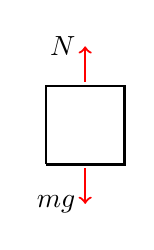
\begin{tikzpicture}
    \draw[thick] (0,0) -- (1,0) -- (1,1) -- (0,1) -- (0,0);
    \draw[thick, ->, color=red] (0.5, -0.05)->(0.5,-0.5);
    \draw (.5,-0.5) node[left] {$mg$};
    \draw[thick, ->, color=red] (0.5, 1.05)->(0.5,1.5);
    \draw (.5,1.5) node[left] {$N$};
    \end{tikzpicture}\\
    A cube of mass $m$ with an acceleration $a$ towards the right and experiencing a frictional force $F$:\\ \\
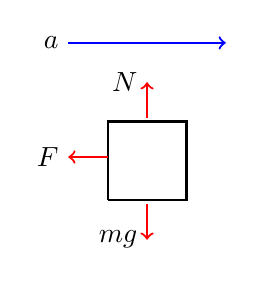
\begin{tikzpicture}
    \draw[thick] (0,0) -- (1,0) -- (1,1) -- (0,1) -- (0,0);
    \draw[thick, ->, color=red] (0.5, -0.05)->(0.5,-0.5);
    \draw (.5,-0.5) node[left] {$mg$};
    \draw[thick, ->, color=red] (0, .55)->(-0.5,0.55);
    \draw (-.5,0.55) node[left] {$F$};
    \draw[thick, ->, color=red] (0.5, 1.05)->(0.5,1.5);
    \draw (.5,1.5) node[left] {$N$};
    \draw[thick, ->, color=blue] (-0.5, 2)->(1.5,2);
    \draw (-0.5,2) node[left] {$a$};
\end{tikzpicture}\\
A point on the top of a roller moving with velocity $v$ towards the right and angular velocity $\omega$:\\
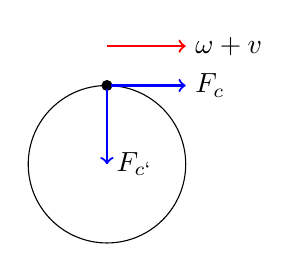
\begin{tikzpicture}
    \draw (1,1) circle (1cm);
    \fill (1,2)  circle[radius=2pt, color=black];
    \draw[thick, ->, color=blue] (1.05, 2)->(2,2);
    \draw (2,2) node[right] {$F_c$};
    \draw[thick, ->, color=blue] (1, 1.95)->(1,1);
    \draw (1,1) node[right] {$F_{c`}$};
    \draw[thick, ->, color=red] (1, 2.5)->(2,2.5);
    \draw (2,2.5) node[right] {$\omega + v$};
\end{tikzpicture}\\
\end{center}
Try thinking through why there is no normal force or weight on the object and also, if you are curious about what $F_c$ and $F_{c`}$ are, they are the centrifugal and centripetal forces. Find which one is which. XD}
\end{phybox}
%-----------------------------------------------------------------
\begin{chembox}{\text{\subsection{What are Subshells and Orbitals?}}}
{\textbf{Subshells:}\\
Each shell is composed of one or more subshells, which are themselves composed of atomic orbitals. For example, the first $(K)$ shell has one subshell, called $1s$; the second $(L)$ shell has two subshells, called $2s$ and $2p$; the third shell has $3s$, $3p$, and $3d$; the fourth shell has $4s$, $4p$, $4d$ and $4f$; the fifth shell has $5s$, $5p$, $5d$, and $5f$ and can theoretically hold more in the $5g$ subshell that is not occupied in the ground-state\footnote{The lowest energy state; i.e when the electron has very less energy to release or absorb.} electron configuration of any known element.
Each subshell is constrained to hold $4l$ + $2$ electrons at most, namely:
\begin{itemize}
    \item {Each $s$ subshell holds at most 2 electrons}
    \item{Each $p$ subshell holds at most 6 electrons}
    \item{Each $d$ subshell holds at most 10 electrons}
    \item{Each $f$ subshell holds at most 14 electrons}
    \item{Each $g$ subshell holds at most 18 electrons}
\end{itemize}
\textbf{Atomic Orbitals:}\\
In atomic theory and quantum mechanics, an atomic orbital is a mathematical function describing the location and wave-like behavior of an electron in an atom.This function can be used to calculate the probability of finding any electron of an atom in any specific region around the atom's nucleus. The term atomic orbital may also refer to the physical region or space where the electron can be calculated to be present, as predicted by the particular mathematical form of the orbital.
Orbitals have been given names, which are usually given in the form:\\
X orbital$^y$; where $X$ is the energy level corresponding to the principal quantum number $n$; type is a lower-case letter denoting the shape or subshell of the orbital, corresponding to the angular quantum number $l$; and $y$ is the number of electrons in that orbital.\\
For example, the orbital $1s^2$ (pronounced as the individual numbers and letters: "'one' 's' 'two'") has two electrons and is the lowest energy level $(n = 1)$ and has an angular quantum number of $l$ = 0, denoted by s.}
\end{chembox}
%------------------------------------------------------------
%------------------------------------------------------------
\begin{mathbox}{\text{\subsection{Modular Arithmetic}}}
{Modular Arithmetic is an operation (used extensively in Mathematical Olympiads and Number Theory) to compute the remainder when a number is divided by another. For example, say $5$ is the remainder when $a$ is divided by $b$. We can represent it the following way:
\begin{align*}
    a \equiv 5 \pmod b
\end{align*}
where $\pmod b$ represents $a$ taken modulo $b$ and $5$ is $a \pmod 5$.\\
Modulos can also be thought of this way. 
\begin{align*}
    14 \equiv 2 \pmod 3
\end{align*}
On adding $3$ to the remainder;   
\begin{align*}
     14 \equiv 5 \pmod 3
\end{align*}
But this is true too (since $14$ leaves a remainder of 5 on being divided by $9$). Are we arriving upon a paradox? No, not at all.
This actually leads us to our next point.\\
A property of congruence systems is that;
\begin{align*}
    \text{If } a \equiv b \pmod n \implies \text{(it implies) } a \equiv b + n \pmod{n}
\end{align*}
Modular Arithmetic systems also have the following properties;
\begin{itemize}
    \item{If $a \equiv b \pmod n$ and $c \equiv d \pmod n;~ab \equiv cd \pmod n$}
    \item{If $a \equiv b \pmod n$ and $c \equiv d \pmod n;~a + b \equiv c + d \pmod n$}
\end{itemize}
The same apply for division and subtraction respectively.}
\end{mathbox}
%------------------------------------------------------------
\begin{phybox}{\text{\subsection{Conservation of Energy}}}
{Conservation of energy, is a principle in physics according to which the energy of interacting bodies or particles in a closed system remains constant. The first kind of energy to be recognized was kinetic energy, or energy of motion. In certain particle collisions, called elastic, the sum of the kinetic energy of the particles before collision is equal to the sum of the kinetic energy of the particles after collision. The notion of energy was progressively widened to include other forms. The kinetic energy lost by a body slowing down as it travels upward against the force of gravity was regarded as being converted into potential energy, or stored energy, which in turn is converted back into kinetic energy as the body speeds up during its return to Earth. For example, when a pendulum swings upward, kinetic energy is converted to potential energy. When the pendulum stops briefly at the top of its swing, the kinetic energy is zero, and all the energy of the system is in potential energy. When the pendulum swings back down, the potential energy is converted back into kinetic energy. This is given as:-
\begin{align*}
    K_1+U_1=K_2+U_2
\end{align*}}
\end{phybox}
%-----------------------------------------------------------------
\begin{chembox}{\text{\subsection{Block Building Principle}}}
{The Aufbau principle, from the German "Aufbauprinzip" (building-up principle), also called the Aufbau rule, states that in the ground state of an atom or ion, electrons fill atomic orbitals of the lowest available energy levels before occupying higher levels. For example, the $1s$ subshell is filled before the $2s$ subshell is occupied. In this way, the electrons of an atom or ion form the most stable electron configuration possible. An example is the configuration $1s^2$ $2s^2$ $2p^6$ $3s^2$ $3p^3$ for the phosphorus atom, meaning that the $1s$ subshell has 2 electrons, and so on.

Electron behavior is elaborated by other principles of atomic physics, such as Hund's rule and the Pauli exclusion principle. Hund's rule asserts that if multiple orbitals of the same energy are available, electrons will occupy different orbitals singly before any are occupied doubly. If double occupation does occur, the Pauli exclusion principle requires that electrons that occupy the same orbital must have different spins. That is $\pm\frac{1}{2}$.
\begin{center}
    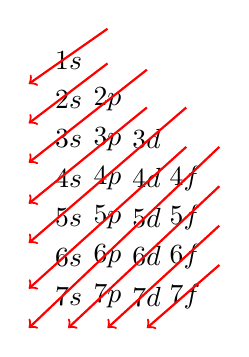
\begin{tikzpicture}
        \draw (-1,3) node[left] {$1s$};
        \draw (-1,2.5) node[left] {$2s$};
        \draw (-1,2) node[left] {$3s$};
        \draw (-1,1.5) node[left] {$4s$};
        \draw (-1,1) node[left] {$5s$};
        \draw (-1,0.5) node[left] {$6s$};
        \draw (-1,0) node[left] {$7s$};
        
        \draw (-0.5,2.5) node[left] {$2p$};
        \draw (-0.5,2) node[left] {$3p$};
        \draw (-0.5,1.5) node[left] {$4p$};
        \draw (-0.5,1) node[left] {$5p$};
        \draw (-0.5,0.51) node[left] {$6p$};
        \draw (-0.5,0) node[left] {$7p$};

        \draw (0,2) node[left] {$3d$};
        \draw (0,1.5) node[left] {$4d$};
        \draw (0,1) node[left] {$5d$};
        \draw (0,0.51) node[left] {$6d$};
        \draw (0,0) node[left] {$7d$};
        
        \draw (.5,1.5) node[left] {$4f$};
        \draw (.5,1) node[left] {$5f$};
        \draw (.5,0.51) node[left] {$6f$};
        \draw (.5,0) node[left] {$7f$};
        
        \draw[thick, ->, color=red] (-0.8, 3.4)->(-1.8,2.7);
        \draw[thick, ->, color=red] (-0.8, 2.96)->(-1.8,2.2);
        \draw[thick, ->, color=red] (-0.3, 2.88)->(-1.8,1.7);
        \draw[thick, ->, color=red] (-0.3, 2.4)->(-1.8,1.18);
        \draw[thick, ->, color=red] (0.2, 2.4)->(-1.8,0.68);
        \draw[thick, ->, color=red] (0.2, 1.9)->(-1.8,0.1);
        \draw[thick, ->, color=red] (0.62, 1.9)->(-1.8,-0.4);
        \draw[thick, ->, color=red] (0.62, 1.4)->(-1.3,-0.4);
        \draw[thick, ->, color=red] (0.62, 0.9)->(-0.8,-0.4);
        \draw[thick, ->, color=red] (0.62, 0.4)->(-0.3,-0.4);
    \end{tikzpicture}
\end{center}
A diagrammatic representation of the order to fill electron subshells.}
\end{chembox}
%------------------------------------------------------------
\begin{mathbox}{\text{\subsection{Quadratic Residues (Not to be residued!)}}}
{An interesting part of modular arithmetic congruence systems is quadratic residues which represent the remainder when a perfect square is divided by some integer $n$. \\
For example, one can observe that $0$ and $1$ are the quadratic residues when any perfect square is taken modulo $4$; i.e.$\pmod 4$.\\
This has a very simple proof. We know that any integer $x$ is either $0, 1, 2$ or $3 \pmod 4$. From the multiplicative property,
\begin{center}
    $x \equiv 0, 1, 2, 3 \pmod 4\\
    \implies x \times x \equiv 0 \times 0, 1 \times 1, 2 \times 2, 3 \times 3 \pmod 4\\
    \implies x \equiv 0, 1, 4, 9 \pmod 4\\
    \text{On writing $4$ and $9$ as $4 + 0$ and $2\times 4 + 1$},\\
    $x$ \equiv 0, 1 \pmod 4$
\end{center}
The following table lists quadratic residues when taken$\pmod n$;
\begin{center}
\begin{tabular}{ |c|c| } 
    \hline
    $n$ & $x^2 \pmod n$\\
    \hline
    $1$ & $0$\\
    $2$ & $0, 1$\\
    $3$ & $0, 1$\\
    $4$ & $0, 1$\\
    $5$ & $0, 1, 4$\\
    $6$ & $0, 1, 3, 4$\\
    $7$ & $0, 1, 2, 4$\\
    $8$ & $0, 1, 4$\\
    \hline
\end{tabular}
\end{center}
Quadratic residues are extensively used to compute Polynomials and i quadratic equations.
\\\\
\textbf{Some Problems! } 
\begin{itemize}
    \item{Can the sum of 2 squares leave a reminder of $3$ when divided by 4?}
    \item{Can the difference of 2 squares be of the form $2(2k+1)$?}
\end{itemize}}
\end{mathbox}
%------------------------------------------------------------
\begin{phybox}{\text{\subsection{Conservative and Non Conservative}}}
{In Potential Energy and Conservation of Energy, any transition between kinetic and potential energy conserved the total energy of the system. This was path independent, meaning that we can start and stop at any two points in the problem, and the total energy of the system—kinetic plus potential at these points are equal to each other. This is characteristic of a conservative force. We dealt with conservative forces in the preceding section, such as the gravitational force and spring force. When comparing the motion of the football}
{The total energy of the system never changes, even though the gravitational potential energy of the football increases, as the ball rises relative to ground and falls back to the initial gravitational potential energy when the football player catches the ball. Non-conservative forces are dissipative forces such as friction or air resistance. These forces take energy away from the system as the system progresses, energy that you can’t get back. These forces are path dependent; therefore it matters where the object starts and stops.}
\end{phybox}
%-------------------------------------------------------------
\begin{chembox}{\text{\subsection{Hund's Choco Orbital Rule}}}
{According to Hund’s rule:

Before the double occupation of any orbital, every orbital in the sub level is singly occupied.
For the maximization of total spin, all electrons in a single occupancy orbital have the same spin.
An electron will not pair with another electron in a half-filled orbital as it has the ability to fill all its orbitals with similar energy. Many unpaired electrons are present in atoms which are at the ground state. If two electrons come in contact they would show the same behaviour as two magnets do. The electrons first try to get as far away from each other as possible before they have to pair up.

The electrons enter an empty orbital before pairing up. The electrons repel each other as they are negatively charged. The electrons do not share orbitals to reduce repulsion.

When we consider the second rule, the spins of unpaired electrons in singly occupied orbitals are the same. The initial electrons spin in the sub-level decides what the spin of the other electrons would be. For instance, a carbon atom’s electron configuration would be $1s^2$ $2s^2$ $2p^2$. The same orbital will be occupied by the two 2s electrons although different orbitals will be occupied by the two $2p$ electrons in reference to Hund’s rule.}
\end{chembox}
%------------------------------------------------------------
\begin{mathbox}{\text{\subsection{Triangle Centers}}}
{There are 4 centers (among the many that are insignificant to us) that are present in a triangle. They are the Centroid, Orthocentre, Circumcenter and Incenter.

\textbf{Centroid: }The centroid is the intersecting point of all the 3 medians of a triangle. It is also the center of mass of a regular (in terms of mass, not equilateral) triangle with a plane surface. Thus, if you place a triangle's centroid on a small point and try to balance it, it will most likely work if your graphing skills are dope like \textbf{Psi25Omega} (Just Kidding) and you ensure no natural factors affect the triangle.

\textbf{Orthocenter: }The orthocentre is the meeting point of all altitudes. It essentially isn't the center of mass but has some special properties that are too overpowered to be discussed here.

\textbf{Circumcenter: }The circumcenter of a triangle is the center of a circle passing through the three vertices of a triangle (the circumscribed circle). It is also the intersection of the perpendicular bisectors of the sides of the triangle.

\textbf{Incenter: }The incenter is the center of the inscribed circle (the circle tangent to the three sides and drawn inside the triangle). It is also incidentally, the intersetion of the angle bisectors of the 3 angles in the triangle.

The centers are usually denoted by these alphabtets;\\
Centroid - G, Orthocenter - H, Circumcenter - O, Incenter - I.

\\
\textbf{Some Special Cases:\footnote{My (Psi25Omega's) \LaTeX ~skills aren't so pro, so I can't draw an illustration for every center.} }
\begin{itemize}
    \item{In the case of a right triangle, the circumcenter is the vertex opposite to the hypotenuse.}
    \item{In an equilateral triangle, all these converge and are basically the same point.}
\end{itemize}
\begin{center}
    Just this one illustration;\\
    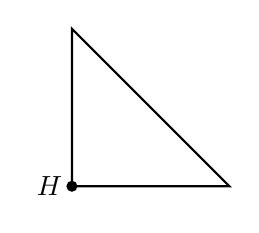
\begin{tikzpicture}
        \draw[thick] (0,0) -- (2,0) -- (0,2) -- (0,0);
        \fill (0,0)  circle[radius=2pt, color=red];
        \draw (0,0) node[left] {$H$};
    \end{tikzpicture}
\end{center}}
\end{mathbox}
%------------------------------------------------------------
\begin{phybox}{\text{\subsection{Thonk about This!}}}
{When it is given that a specific pulley is mass less then the tensions on both the sides of that pulley are equal.

If you encounter with a situation as shown in the below picture and if the pulley is mass-less, then the the tension on both sides are equal; i.e.
\begin{center}
    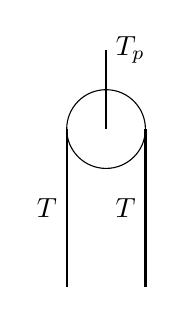
\begin{tikzpicture}
        \draw (0,0) circle (0.5cm);
        \draw[thick] (0,0) -- (0,1);
        \draw[thick] (0.5,0) -- (0.5,-2);
        \draw[thick] (-0.5,0) -- (-0.5,-2);
        \draw (0,1) node[right] {$T_p$};
        \draw (0.5,-1) node[left] {$T$};
        \draw (-0.5,-1) node[left] {$T$};
    \end{tikzpicture}
\end{center}
\begin{align*}
    2T_p = T+T = 2T
\end{align*}
There are many such conditions and situations under which you can equate tension in different places in a pulley-system. Pulleys are also called the Atwood's Machine. There's also the concept of "slack" to calculate the magnitude of acceleration that bodies in a pulley system when they are released - left to free fall. But there's a nice formula to calculate the force and the acceleration for a 2-body system.
\begin{center}
    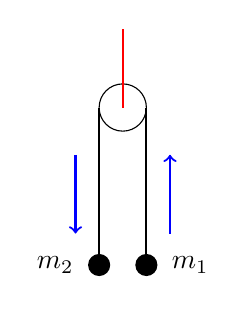
\begin{tikzpicture}
        \draw (0,0) circle (0.3cm);
        \draw[thick, color=red] (0,0) -- (0,1);
        \draw[thick] (0.3,0) -- (0.3,-2);
        \draw[thick] (-0.3,0) -- (-0.3,-2);
        \draw (0.5,-2) node[right] {$m_1$};
        \fill (0.3,-2)  circle[radius=4pt, color=black];
        \fill (-0.3,-2)  circle[radius=4pt, color=black];
        \draw (-0.5,-2) node[left] {$m_2$};
        \draw[thick, ->, color=blue] (0.6, -1.6)->(0.6, -0.6);
        \draw[thick, ->, color=blue] (-0.6, -0.6)->(-0.6, -1.6);
    \end{tikzpicture}
\end{center}
Let's say the acceleration of both the blocks is $a$ (it is gonna be the same except for the direction).

Then the tension in the string $T$ is given by
\begin{align*}
    T = \frac{2m_1m_2g}{m_1+m_2}
\end{align*}
while the acceleration $a$\footnote{Here, consider $m_2 > m_1$ and the direction of acceleration of block with mass $m_1$ as positive. (Also, try deriving these on your own with an FBD)} is given by
\begin{align*}
    a = \frac{(m_2-m_1)g}{m_1+m_2}
\end{align*}}
\end{phybox}
%-----------------------------------------------------------
\begin{chembox}{\text{\subsection{Pauli's "Excluded" Principle}}}
{The Pauli's exclusion principle is the quantum mechanical principle which states that two or more identical fermions\footnote{Particles with half-integer spin} cannot occupy the same quantum state within a quantum system simultaneously. This principle was formulated by Austrian physicist Wolfgang Pauli in 1925 for electrons, and later extended to all fermions with his spin–statistics theorem of 1940.
In the case of electrons in atoms, it can be stated as follows: it is impossible for two electrons of a poly-electron atom to have the same values of the four quantum numbers: $n$, the principal quantum number, $l$, the azimuthal quantum number, $m$, the magnetic quantum number, and $s$, the spin quantum number. For example, if two electrons reside in the same orbital, then their $n$, $l$, and $m$ values are the same, therefore their $s$ must be different, and thus the electrons must have opposite half-integer spin projections of $\frac{1}{2}$ and $-\frac{1}{2}$.}
\end{chembox}
%-------------------------------------------------------------
\begin{mathbox}{\text{\subsection{GCD and 2 Proofs}}}
{The GCD (Greatest Common Divisor) of 2 or more numbers is the largest integer that divides all of the numbers. There are a few properties GCD has and we can exploit them to prove lemmas among others.

For 2 numbers $a$ and $b$;
\begin{align*}
    \gcd(a,b) = \gcd(a-b, b)
\end{align*}
This is also heavily used in the result of the Euclidean Division Algorithm. 

\textbf{Proof:}\\
Let's assume 
\begin{align*}
    \gcd(a,b) = k
\end{align*} where $k$ is any integer and let 
\begin{align*}
    a = ka' \text{ and } b = kb'
\end{align*}
From this, 
\begin{align*}
    a-b = k(a'-b')
\end{align*}
Notice that this is also divisible by $k.$ \\
This proves the statement and wait, we have a problem!
\\\\
\textbf{IMO 1959 P1:} Prove that the fraction $\frac{21n+4}{14n+3}$ is irreducible (cannot be simplified further) for every natural number $n$.\footnote{Here, we essentially need to prove $\gcd(21n+4, 14n+3) = 1$}
\\\\
A special relation between the LCM and GCD of 2 numbers exists;
\begin{align*}
    \lcm(a,b) \cdot \gcd(a,b) = ab
\end{align*}
The proof involves some prime factorization of the $\gcd$ combined with some manipulation.}
\end{mathbox}
%------------------------------------------------------------
\begin{phybox}{\text{\subsection{Pulleys, MA and Planes!}}}
{\textbf{Pulleys}
A pulley is a wheel on an axle or shaft that is designed to support movement and change of direction of a taut cable or belt, or transfer of power between the shaft and cable or belt. In the case of a pulley supported by a frame or shell that does not transfer power to a shaft, but is used to guide the cable or exert a force, the supporting shell is called a block, and the pulley may be called a sheave.

A pulley may have a groove or grooves between flanges around its circumference to locate the cable or belt. The drive element of a pulley system can be a rope, cable, belt, or chain.

It can be of three types
\begin{itemize}
    \item {\textbf{Fixed}:A fixed pulley has an axle mounted in bearings attached to a supporting structure. A fixed pulley changes the direction of the force on a rope or belt that moves along its circumference. Mechanical advantage is gained by combining a fixed pulley with a movable pulley or another fixed pulley of a different diameter.}
    \item {\textbf{Movable}:A movable pulley has an axle in a movable block. A single movable pulley is supported by two parts of the same rope and has a mechanical advantage of two.}
    \item {\textbf{Compound}:A combination of fixed and movable pulleys forms a block and tackle. A block and tackle can have several pulleys mounted on the fixed and moving axles, further increasing the mechanical advantage.}
 \end{itemize}   

\textbf{Inclined Planes}
An inclined plane, also known as a ramp, is a flat supporting surface tilted at an angle, with one end higher than the other, used as an aid for raising or lowering a load.
Due to conservation of energy, the same amount of mechanical energy (work) is required to lift a given object by a given vertical distance, disregarding losses from friction, but the inclined plane allows the same work to be done with a smaller force exerted over a greater distance.
The angle of friction, also sometimes called the angle of repose, is the maximum angle at which a load can rest motionless on an inclined plane due to friction, without sliding down. This angle is equal to the arctangent of the coefficient of static friction μs between the surfaces.

The mechanical advantage of an inclined plane depends on its slope, meaning its gradient or steepness. The smaller the slope, the larger the mechanical advantage, and the smaller the force needed to raise a given weight. A plane's slope $s$ is equal to the difference in height between its two ends, or "rise", divided by its horizontal length, or "run".This can be also said as:
\begin{align*}
  \theta = \tan^-1 \frac{Rise}{Run}  
\end{align*}

\textbf{Mechanical Advantage}
The mechanical advantage MA of a simple machine is defined as the ratio of the output force exerted on the load to the input force applied. For the inclined plane the output load force is just the gravitational force of the load object on the plane, its weight $F_w$. The input force is the force $F_i$ exerted on the object, parallel to the plane, to move it up the plane. The mechanical advantage is
\begin{align*}
    MA= \frac{F_w}{F_i}
\end{align*}}
\end{phybox}
%------------------------------------------------------------
\begin{chembox}{\text{\subsection{A Salty Bond}}}
{The {Ionic bond} is a type of a {chemical bond} that is a result of the attraction {between oppositely charged particles} in ionic compounds like NaCl\footnote{More examples; KCl, CaCl_2}. Ions are atoms (or a group of atoms) having a {net charge}. Atoms that {gain electrons} to become {stable} are called {anions} while those that {lose electrons} for the same are called {cations}. This {transfer of electrons} is known as {electrovalence}. Ionic bonds are {mostly} formed {between metals and non-metals}. In simpler words, an ionic bond is a result of the transfer of electrons from a metal (cation) to a non-metal (anion) in order for both atoms to attain stability.

It is important to recognize that clean ionic bonding — in which one atom or molecule completely transfers an electron to another — cannot exist: all ionic compounds have some degree of covalent bonding (where electron pairs are shared), or electron sharing. Thus, the term "ionic bonding" is given when the ionic character is greater than the covalent character.

Ionic compounds conduct electricity when molten or in dissolved in a solvent, typically not when solid. Ionic compounds generally have a high melting point because the bond is ironically very strong, though held by just electron clouds and the attraction. Depending on the charge of the ions they consist of, higher charges mean stronger cohesive forces and a higher melting point. They also tend to be soluble in water; and the stronger the cohesive forces, the lower the solubility.

Here is an example of an ionic bond between Na\footnote{The green one} and Cl\footnote{The blue one}.
\begin{center}
    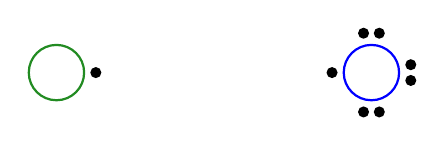
\begin{tikzpicture}
        \draw[thick, ForestGreen] (-2,0) circle (10pt);
        \fill (-1.5,0)  circle[radius=2pt, color=black];
        \draw[thick, blue] (2,0) circle (10pt);
        \fill (1.5,0)  circle[radius=2pt, color=black];
        \fill (1.9,.5)  circle[radius=2pt, color=black];
        \fill (2.1,.5)  circle[radius=2pt, color=black];
        \fill (2.5,.1)  circle[radius=2pt, color=black];
        \fill (2.5,-0.1)  circle[radius=2pt, color=black];
        \fill (1.9,-.5)  circle[radius=2pt, color=black];
        \fill (2.1,-.5)  circle[radius=2pt, color=black];
    \end{tikzpicture}
\end{center}
\\
\\
\begin{center}
    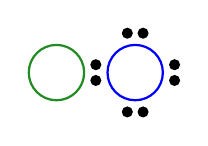
\begin{tikzpicture}
        \draw[thick, ForestGreen] (-.5,0) circle (10pt);
        \fill (0,0.1)  circle[radius=2pt, color=black];
        \fill (0,-0.1)  circle[radius=2pt, color=black];
        \draw[thick, blue] (.5,0) circle (10pt);
        \fill (0.4,.5)  circle[radius=2pt, color=black];
        \fill (0.6,.5)  circle[radius=2pt, color=black];
        \fill (1,.1)  circle[radius=2pt, color=black];
        \fill (1,-0.1)  circle[radius=2pt, color=black];
        \fill (0.4,-.5)  circle[radius=2pt, color=black];
        \fill (0.6,-.5)  circle[radius=2pt, color=black];
    \end{tikzpicture}
\end{center}
Here, the black dots represent the electrons.}
\end{chembox}
%-------------------------------------------------------------
\begin{phybox}{\text{\subsection{Constraint Relation}}}
{Constraint Relation is a beautiful and interesting concept which helps in solving questions related to pulleys and strings. It can be used to solve even the most complicated problems. Once understood it will be a very useful tool in solving problems in dynamics.

Constraint relation says that the sum of products of all tensions in strings and velocities of respective blocks connected to the strings is equal to $0$. In other words it says that the total power by tension is zero. Mathematically it is represented by :
\begin{align*}
\displaystyle \sum T \cdot \Vec{v} = 0
\end{align*}

If the velocity vector is constant then differentiating the above equation with respect to time we get another relation. If the velocity vector is constant then the sum of products of all tensions in strings and accelerations of respective blocks connected to the strings is equal to 00. It is mathematically represented by :
\begin{align*}
    \displaystyle \sum T \cdot \Vec{a} = 0
\end{align*}

\textbf{Note}: Constraint relation works only when the strings are inextensible and taut.}
\end{phybox}
%-----------------------------------------------------------
\begin{guidebox}{A Clarification}
{We skipped Math on the 31st and interchanged it with Physics because we felt it would be a sin to move Constraint Relation to February as it the month has a completely different outlook and context.\footnote{OK! Considering it a sin is an exaggeration but yeah, moving it would cause unneeded confusion and we needed to break the arbitrariness of the schedule to do so.}}
\end{guidebox}
%-----------------------------------------------------------
\newpage
%-----------------------------------------------------------
